\documentclass[12pt, a4paper, oneside]{ctexart}
\usepackage{amsmath, amsthm, amssymb, bm, color, framed, graphicx, hyperref, mathrsfs}
\usepackage[inline]{enumitem}
\usepackage{tikz}
\usepackage{pgfplots}
\pgfplotsset{compat=1.16}

\title{\textbf{多元统计分析课程作业3}}
\author{Phlins}
\date{\today}
\linespread{1.5}
\definecolor{shadecolor}{RGB}{241, 241, 255}
\newcounter{problemname}
\newenvironment{problem}{\begin{shaded}\stepcounter{problemname}\par\noindent\textbf{题目\arabic{problemname}. }}{\end{shaded}\par}
\newenvironment{solution}{\par\noindent\textbf{解答. }}{\par}
\newenvironment{note}{\par\noindent\textbf{题目\arabic{problemname}的注记. }}{\par}

\begin{document}

\maketitle

\begin{problem}
    5.1
    \begin{enumerate}[label=(\alph*)]
        \item 使用给定的数据计算检验统计量 $T^{2}$ 以检验原假设 $H_{0} \colon \mu^{\prime}= [7,11]$,
        $$
        \mathbf{X}= \begin{bmatrix} {2} & {12} \\ {8} & {9} \\ {6} & {9} \\ {8} & {10} \\ \end{bmatrix}
        $$
        \item 描述(a)部分中 $T^{2}$ 统计量的分布情况。
        \item 结合(a)和(b)的结果,在 $\alpha=0.05$ 的显著性水平下对原假设 $H_{0}$ 进行检验。你会得出什么结论?
    \end{enumerate}
\end{problem}


\begin{solution}
    \begin{enumerate}[label=(\alph*)]
        \item 
        \begin{gather*}
            \text{变量数}p=2,\text{样本大小}n=4\\
            \bar{x}=\begin{bmatrix}
                \frac{2+8+6+8}{n}\\
                \frac{12+9+9+10}{n}
            \end{bmatrix}
            =\begin{bmatrix}
                6\\
                10
            \end{bmatrix},\\
            S_{ij} = \frac{1}{n-1} \sum_{k=1}^{n} (x_{ki} - \bar{x}_i)(x_{kj} - \bar{x}_j) ,
            \mathbf{S}=\begin{bmatrix}
                8 & -\frac{10}{3}\\
                -\frac{10}{3} & 2
            \end{bmatrix},\\
            T^{2}=n(\bar{x} - \mu^\prime)^\top \mathbf{S}^{-1} (\bar{x} - \mu^\prime)=\frac{150}{11}=13.64
        \end{gather*}
        \item 
        \begin{gather*}
            \because T^{2} \sim \frac{( n-1 ) p} {( n-p )} F_{p, n-p},\\
            \therefore T^{2} \sim 3F_{2,2}
        \end{gather*}
        \item 
        \begin{gather*}
            H_{0} \colon \mu^{\prime}= [7,11]\\
            \because \alpha=0.05 \therefore F_{2,2}(0.05)=19\\
            \because T^{2}=13.64<3F_{2,2}(0.05)=57\\
            \therefore \alpha=0.05\text{时接受原假设} H_{0}
        \end{gather*}

      \end{enumerate}
\end{solution}



\begin{problem}
5.5.
样本均值向量:
$$
\mathbf{\bar{x}} =
\begin{bmatrix}
0.564 \\
0.603
\end{bmatrix}
$$

样本协方差矩阵:
$$
\mathbf{S} =
\begin{bmatrix}
0.0144 & 0.0117 \\
0.0117 & 0.0146
\end{bmatrix}
$$

样本协方差矩阵的逆矩阵:
$$
\mathbf{S}^{-1} =
\begin{bmatrix}
203.018 & -163.391 \\
-163.391 & 200.228
\end{bmatrix}
$$
在0.05的显著性水平上,对原假设 $H_{0}$ 进行检验,其中原假设为:$H_{0} \colon\boldsymbol{\mu}^{\prime} = [0.55,0.60]$。检验的结果是否与图5.1中所示的 $\boldsymbol{\mu}$ 参数95\%的置信椭圆相一致?请对此进行解释。
\end{problem}

\begin{solution}
    \begin{gather*}
        H_{0} \colon\boldsymbol{\mu}^{\prime} = [0.55,0.60],T^{2}=n(\bar{x} - \mu^\prime)^\top \mathbf{S}^{-1} (\bar{x} - \mu^\prime)=1.17\\
        \alpha=0.05 \therefore F_{2,40}(0.05)=3.23\\
        \because T^{2}=1.17<\frac{2(40+1)}{40},F_{2,40}(0.05)=2.05\times3.23=6.62\\   
    \end{gather*}
    在0.05的显著性水平上,我们不拒绝原假设$H_0$。这一结果与图中所示的95\%置信椭圆一致,因为均值向量$\boldsymbol{\mu}^\prime=[0.55,0.60]$位于该椭圆内部。
    
    \begin{center}
        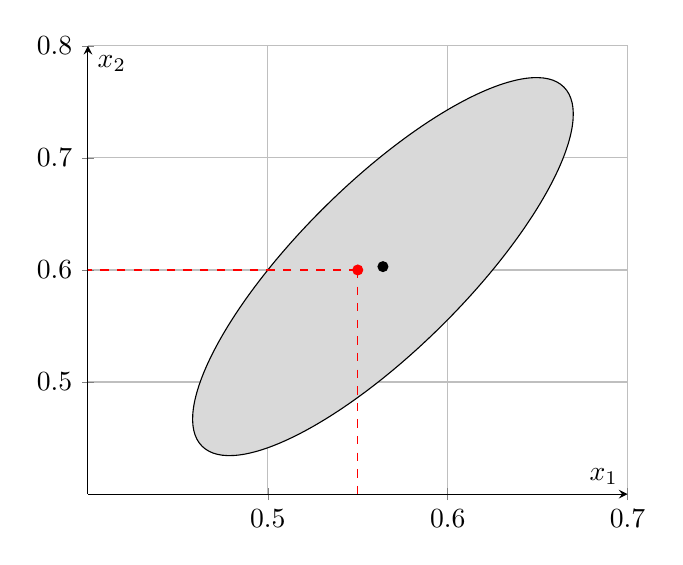
\begin{tikzpicture}
            \begin{axis}[
                xmin=0.4, xmax=0.7,
                ymin=0.4, ymax=0.8,
                axis lines=center,
                xlabel=$x_1$,
                ylabel=$x_2$,
                xtick={0.4,0.5,...,0.7},
                ytick={0.4,0.5,...,0.8},
                grid=major,
            ]
            % Draw the ellipse
            \draw[black, fill=gray!30, rotate around={-135.2448477965646:(0.564, 0.603)}] (0.564, 0.603) ellipse (3.2373092124554926cm and 1.0582197611795cm); 
            % 半长轴长度(major axis): 0.052910988058975*20
            % 半短轴长度(minor axis): 0.16186546062277463*20
            % 旋转角度(degrees): -135.2448477965646
            % 中心坐标(center): [[0.564] [0.603]]

            % Draw the center of the ellipse
            \fill[black] (0.564, 0.603) circle (2pt);
            % Draw the mu point
            \fill[red] (0.55, 0.60) circle (2pt);
            % Draw the dashed lines
            \draw[dashed, red] (0.55, 0.60) -- (0.55, 0);
            \draw[dashed, red] (0.55, 0.60) -- (0, 0.60);
            \end{axis}
        \end{tikzpicture}       
    \end{center}

\end{solution}

\begin{problem}
    绘制散点图,展示当显著性水平 $\alpha=0.05$ 时,对于不同的样本量 $n$(从 2 到 120,步长为 1)和不同自由度 $p$(从 1 到 60,步长为 1)条件下,变量
    $
    \frac{( n-1 ) p} {n-p} F_{p, n-p} ( \alpha)
    $
    的观测值分布情况。
\end{problem}

\begin{solution}
    \begin{figure}[h]
        \centering
        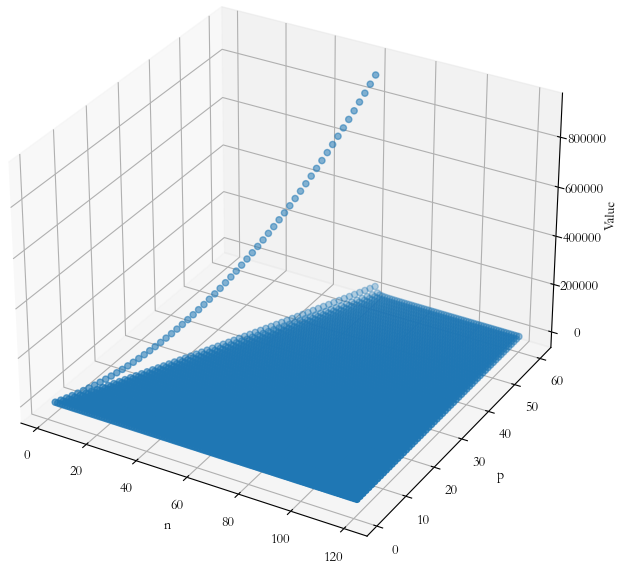
\includegraphics[width=\textwidth]{Assignment3-Figure_1.png}
        \caption{观测值分布情况}
    \end{figure}
\end{solution}


\end{document}